% !TEX root = Anhang.tex

\anhangstart

\begin{figure}[H]
	\centering
	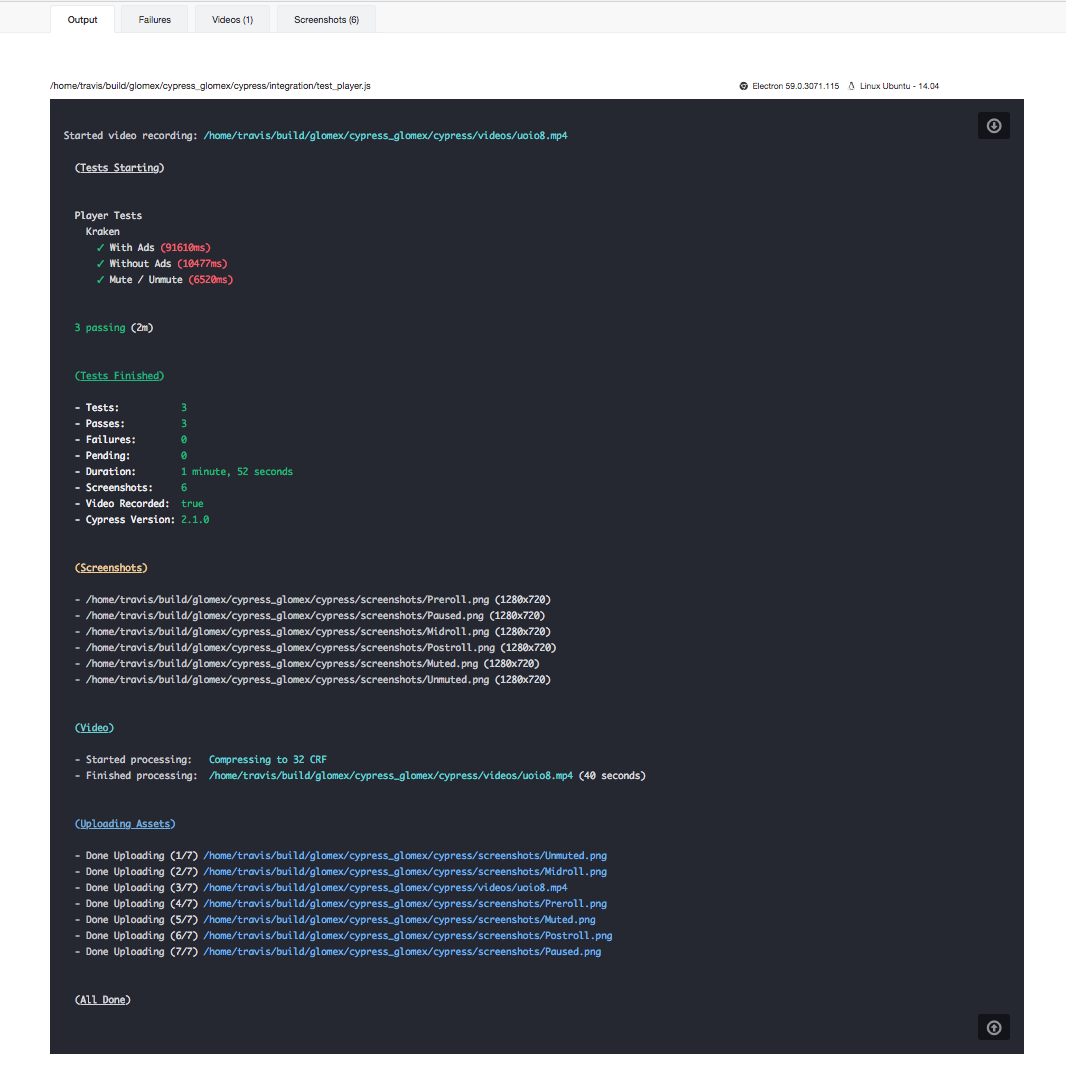
\includegraphics[width=1.0\textwidth]{06_Bilder/Anhang_testdetail_output.png}
	\setlength{\abovecaptionskip}{-1em}
	\caption[]{Anhang Testdetail Output}
	\label{img:anhang_testdetail_output}
\end{figure}

\begin{figure}[H]
	\centering
	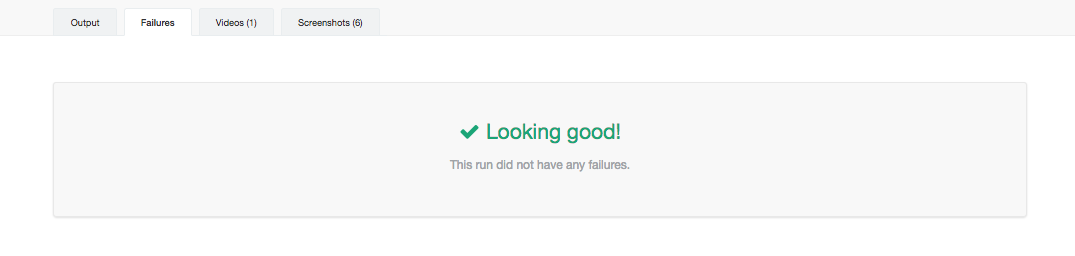
\includegraphics[width=1.0\textwidth]{06_Bilder/Anhang_testdetail_failures.png}
	\setlength{\abovecaptionskip}{-1em}
	\caption[]{Anhang Testdetail Failures}
	\label{img:anhang_testdetail_failures}
\end{figure}

\begin{figure}[H]
	\centering
	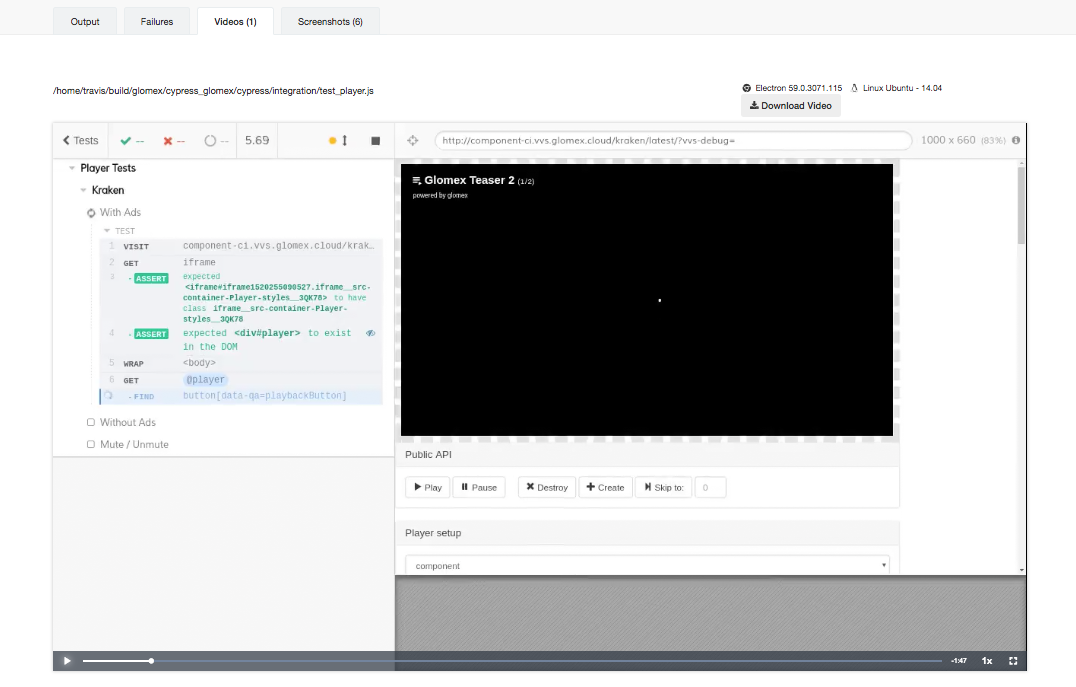
\includegraphics[width=1.0\textwidth]{06_Bilder/Anhang_testdetail_videos.png}
	\setlength{\abovecaptionskip}{-1em}
	\caption[]{Anhang Testdetail Videos}
	\label{img:anhang_testdetail_videos}
\end{figure}

\begin{figure}[H]
	\centering
	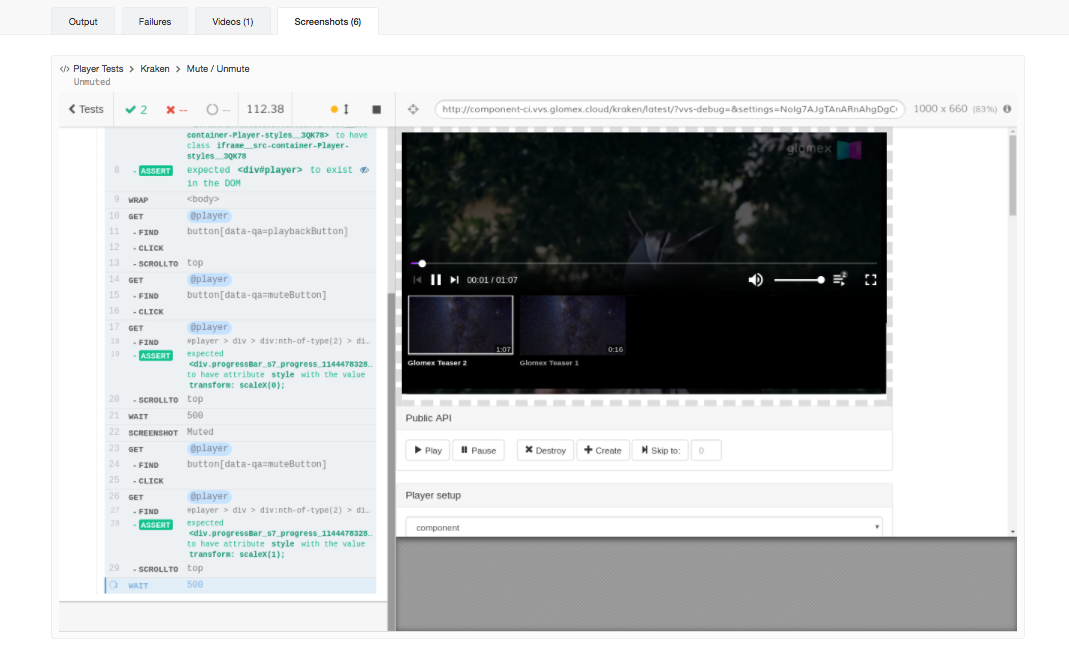
\includegraphics[width=1.0\textwidth]{06_Bilder/Anhang_testdetail_screenshots.png}
	\setlength{\abovecaptionskip}{-1em}
	\caption[]{Anhang Testdetail Screenshots}
	\label{img:anhang_testdetail_screenshots}
\end{figure}

\newpage

	\lstset{style=cypress, caption={test\_player.js, l�uft derzeit (07.03.2018) aktiv auf dem Travis}, label={lst:anhang_test_player}}
\begin{lstlisting}
describe('Player Tests', function() {

/**
* Get all the pre-stuff before every Test
*/
beforeEach(function(){
	cy.fixture('kraken/locators.json').as('locator')
	cy.fixture('kraken/web.json').as('web')
	cy.fixture('kraken/settings.json').as('setting')

})

context('Kraken', function(){

	/**
	* Krakentest with Ads
	*/
	it('With Ads', function(){

		const loc = this.locator
		const time = 10000

		// Visit the Website
		cy.visit(this.web.krakenUrl)

		// find the iFrame
		cy.iframe(loc.playerIframe, "#player")
			.as('player')

		// play the Video
		cy.get("@player")
			.find(loc.playButton, {timeout: time})
			.click()

		// scroll to top
		cy.scrollTo('top')
		
		// is the Ad displaying?
		cy.get("@player").find(loc.adDisclaimer, {timeout: time}) 
		cy.wait(2000).screenshot('Preroll')

		 // is the Video resuming after ad?
		cy.get("@player").find(loc.pauseButton, {timeout: time})

		// Test if the Video is playing
		cy.get("@player").find(loc.videoTimePassed)
			.contains("00:05", {timeout: 10000})

		// Test if pause is working
		cy.get("@player").find(loc.pauseButton).click()
		cy.get("@player").find(loc.playButtonBig)
			.should('be.visible')
		cy.scrollTo('top')
		cy.wait(1000).screenshot('Paused')
		cy.get("@player").find(loc.pauseButton).click()
		cy.scrollTo('top')

		// Test if Midroll is playing
		cy.get("@player")
			.find(loc.adDisclaimer, {timeout: 50000})
		cy.wait(2000).screenshot('Midroll')
		cy.get("@player")
			.find(loc.pauseButton, {timeout: time})

		// Test if Preroll is playing
		cy.get("@player")
			.find(loc.adDisclaimer, {timeout: 50000})
		cy.wait(2000).screenshot('Postroll')
	})
	
	/**
	* Krakentest without Ads
	*/
	it('Without Ads', function(){

		const loc = this.locator
		const time = 10000

		// Visit the Website and deactivate Hornet
		cy.visit(this.web.krakenUrl)
		cy.de_activate_hornet()

		// Find the iFrame
		cy.iframe(loc.playerIframe, "#player").as('player')
		
		// Play the Video
		cy.get("@player").find(loc.playButton).click()
		
		// Scroll to Top
		cy.scrollTo('top')

		// Test if the Video is playing
		cy.get("@player").find(loc.videoTimePassed)
			.contains("00:05", {timeout: time})

		// Test if pause is working
		cy.get("@player").find(loc.pauseButton).click()
		cy.get("@player").find(loc.playButtonBig)
			.should('be.visible')
		cy.scrollTo('top') // scroll to top
	})

	/**
	* Krakentest without Ads and Muted / Unmuted
	*/
	it('Mute / Unmute', function(){

		const loc = this.locator
		const time = 5000

		// Visit the Website and deaktivate Hornet
		cy.visit(this.web.krakenUrl)
		cy.de_activate_hornet()

		// Find the iFrame
		cy.iframe(loc.playerIframe, "#player").as('player')
		
		// Play the Video
		cy.get("@player").find(loc.playButton).click()
		
		// Scroll to Top
		cy.scrollTo('top')

		// Test if the Mute Button works
		cy.get("@player").find(loc.volumeButton).click()
		cy.get("@player").find(loc.volumeBar)
			.should('have.attr', 'style', 'transform: scaleX(0);')
		cy.scrollTo('top') // scroll to top
		cy.wait(500).screenshot('Muted')

		// Test if the Unmute Button works
		cy.get("@player").find(loc.volumeButton).click()
		cy.get("@player").find(loc.volumeBar)
			.should('have.attr', 'style', 'transform: scaleX(1);')
		cy.scrollTo('top') // scroll to top
		cy.wait(500).screenshot('Unmuted')
	})
})
})
\end{lstlisting} 

\newpage

	\lstset{style=cypress, caption={fixtures/kraken/locators.json}, label={lst:locators}}
\begin{lstlisting}
{
"playerIframe": "iframe__src-container-Player-styles__3QK78",
"playButton": "button[data-qa=playbackButton]",
"pauseButton": "button[data-qa=playbackButton]",
"playListButton": "button[data-qa=playlistButton]",
"pauseButton": "button[data-qa=playbackButton]",
"fullscreenButton": "button[data-qa=fullscreenButton]",
"volumeButton": "button[data-qa=muteButton]",
"adDisclaimer": "#player > div > div:nth-of-type(2) 
	> div:nth-of-type(2) > div > div > div > div 
	> div:nth-of-type(5) > div > div:nth-of-type(1) 
	> div:nth-of-type(1) > div > div > strong",
"videoTimePassed": "#player > div > div:nth-of-type(2) 
	> div:nth-of-type(2) > div > div > div > div 
	> div:nth-of-type(5) > div > div:nth-of-type(2) 
	> div:nth-of-type(1) > div > span",
"playButtonBig": "#player > div > div:nth-of-type(2) 
	> div:nth-of-type(2) > div > div > div > div 
	> div:nth-of-type(4) > div:nth-of-type(2) > div 
	> div > button"
"volumeBar": "#player > div > div:nth-of-type(2) 
	> div:nth-of-type(2) > div > div > div > div 
	> div:nth-of-type(5) > div > div:nth-of-type(2) 
	> div:nth-of-type(3) > div:nth-of-type(1) > div 
	> div > div:nth-of-type(1)"
}
\end{lstlisting} 

	\lstset{style=cypress, caption={fixtures/kraken/settings.json}, label={lst:settings}}
\begin{lstlisting}
{
"delay": 20000
}
\end{lstlisting} 

	\lstset{style=cypress, caption={fixtures/kraken/web.json}, label={lst:web}}
\begin{lstlisting}
{
"krakenUrl": "LINK ZUR KRAKEN TESTPAGE"
}
\end{lstlisting} 

	\lstset{style=cypress, caption={support/commands.js}, label={lst:commands}}
\begin{lstlisting}
Cypress.Commands.add('de_activate_hornet', () => {

cy.get('#hornet-input').click()
cy.scrollTo('top')
cy.reload()

})

Cypress.Commands.add('iframe', 
(locator, element, wait=10000) => {

return cy.get('iframe',  { timeout: wait })
.should('have.class', locator)
.should(($iframe) => {
expect($iframe.contents().find(element)).to.exist
}).then(($iframe) => {
return cy.wrap($iframe.contents().find("body"))
});

})
\end{lstlisting} 
